\documentclass[12pt,letterpaper]{article} % use larger type; default would be 10pt

\usepackage[margin=0.8in]{geometry}
\linespread{1.25}

\usepackage[sc]{mathpazo}

\usepackage[english]{babel}
%\usepackage[utf8x]{inputenc}
\usepackage[T1]{fontenc}
\usepackage{tabularx,ragged2e,booktabs,caption}
\usepackage{graphicx}
\usepackage{float}
%\usepackage{tabu}
\usepackage{multirow}

\usepackage{amssymb}

\usepackage{epstopdf}
\usepackage{rotating}
\usepackage{lscape}

\newcommand\fnsep{\textsuperscript{,}}

%\usepackage{csquotes}
\usepackage[toc,page]{appendix}
\usepackage[round]{natbib}
\usepackage{booktabs}   % for nice tables
\usepackage{kpfonts}    % for nice fonts
\usepackage{microtype}
\usepackage[T1]{fontenc}
\usepackage{listings}   % for inserting code
\usepackage{paralist} % very flexible & customisable lists (eg. enumerate/itemize, etc.)
\usepackage{verbatim} % adds environment for commenting out blocks of text & for better verbatim
%\usepackage{subfig} % make it possible to include more than one captioned figure/table in a single float
\usepackage{fancyhdr} % This should be set AFTER setting up the page geometry
\usepackage{caption}
\usepackage{subcaption}
\usepackage{float}
\usepackage{color}  
\usepackage[colorlinks=true]{hyperref}
% use for hypertext

% maths
\usepackage{mathtools}
\usepackage{amsthm}
\usepackage{amsmath}
\usepackage{amssymb}
\usepackage{bbm}
\usepackage{tikz}
\newcommand{\Mypm}{\mathbin{\tikz [x=1.4ex,y=1.4ex,line width=.1ex] \draw (0.0,0) -- (1.0,0) (0.5,0.08) -- (0.5,0.92) (0.0,0.5) -- (1.0,0.5);}}
\newcommand{\R}{\mathbb{R}} 
\newtheorem*{mydef}{Definition}
\pagestyle{fancy} % options: empty , plain , fancy
\renewcommand{\headrulewidth}{0pt} % customise the layout...
\lhead{}\chead{}\rhead{}
\lfoot{}\cfoot{\thepage}\rfoot{}
\DeclareMathOperator*{\argmax}{arg \, max}
\DeclareMathOperator*{\argmin}{arg \, min}
\DeclareMathOperator*{\var}{var}
\DeclareMathOperator*{\cov}{cov}

% proposition, definition, ...
\theoremstyle{plain}
\newtheorem{definition}{Definition}
\newtheorem{theorem}{Theorem}
\newtheorem{proposition}{Proposition}
\newtheorem{lemma}{Lemma}
\newtheorem{corollary}{Corollary}
\newtheorem{remark}{Remark}
\theoremstyle{definition}
\newtheorem{assumption}{Assumption}

\graphicspath{{figures/}}

\usepackage{cleveref} % for clever ref 
\usepackage{array} % for better arrays (eg matrices) in maths
\usepackage{datetime2}
\usepackage{qtree}


\usepackage{hyperref}
\hypersetup{
	colorlinks   = true,
	linkcolor    = black,
	citecolor    = black,
	urlcolor 	 = black,
}
\urlstyle{same}

%%% SECTION TITLE APPEARANCE
\usepackage{sectsty}
\allsectionsfont{\sffamily\mdseries\upshape} % (See the fntguide.pdf for font help)
\usepackage[nottoc,notlof,notlot]{tocbibind} % Put the bibliography in the ToC
\usepackage[titles,subfigure]{tocloft} % Alter the style of the Table of Contents
\renewcommand{\cftsecfont}{\rmfamily\mdseries\upshape}
\renewcommand{\cftsecpagefont}{\rmfamily\mdseries\upshape} % No bold!

\author{ \textsc{Jonathan Créchet}\thanks{Department of Economics, University of Ottawa, 75 Laurier Ave E, K1N 9A6, Ontario, Canada; email: jcrechet@uottawa.ca.} }

\title{A Model of Risk Sharing in a Dual Labor Market - Tables and Figures}

\date{October 2024}

\begin{document}
	
	\maketitle

	\begin{abstract}
		In OECD countries, the labor market features a coexistence of open-ended, permanent jobs subject to strict employment protection and fixed-term, temporary jobs. This paper studies a search-and-matching model with risk-averse workers and dynamic employment contracts subject to limited commitment. In equilibrium, permanent and temporary jobs coexist when the match quality is sufficiently dispersed: firing costs generate insurance gains implying that permanent contracts are optimal for high-quality matches. Consistent with recent empirical evidence, quantitative analysis of the model shows that temporary contracts crowd out permanent jobs and do not generate employment gains.
	\end{abstract}
	
	\noindent \textbf{JEL Codes}: E24, J41, J58
	
	\smallskip
	
	\noindent \textbf{Keywords}: Search frictions, Dynamic contracts, Limited commitment, Employment protection legislation.
	
	\newpage
	
	\begin{table}[!h]
	\centering
	\captionof{table}{Benchmark parameter values}
	\label{tab:param:benchmark}
	\begin{tabular}{l l c}
		\hline \hline
		\addlinespace
		\textit{Preset} & & \\ 
		$\beta$ & Discount factor & 0.996 \\ 
		$\sigma$ & Relative risk aversion & 2.5 \\ 
		$\eta$ & Elasticity of matching & 0.5 \\ 
		$\gamma$ & Worker's bargaining power & 0.5 \\ 
		$\delta$ & Exogenous separation probability & 0.0024 \\ 
		$F$ & Firing costs & 0 \\ 
		\addlinespace
		\textit{Internal} & & \\ 
		$b$ & Non-work income & 0.383 \\ 
		$A$ & Matching efficiency & 0.600 \\ 
		$\lambda$ & Probability of idiosyncratic shock & 0.068 \\ 
		$\sigma_x^2$ & Log match-quality variance & 0.204 \\ 
		$\mu_x$ & Log match-quality mean & -0.102 \\ 
		$\kappa$ & Vacancy posting cost & 2.096 \\ 
		\addlinespace
		\hline \hline
	\end{tabular}
	\caption*{\footnotesize Notes: Parameter values in the benchmark U.S.\ calibrated economy. The exogenous probability of separation $\delta$ is set following \cite{jung_kuhn:JEEA:2019}. The other preset parameters are standard. The targets for the internally calibrated parameters are an unemployment rate equal to 5.6\%, an aggregate EU probability of 2\%, non-work income $b=0.4$ (\cite{shimer:2005:AER}), and relative separation rates by tenure estimated from the Job Tenure Supplement of the CPS (less than one year of tenure to 1-15 years). Moreover, $\mu_x = -\sigma_x^2/2$. The value of $\kappa$ is set to be consistent with the normalization that labor-market tightness $\theta=1$ (\cite{shimer:2005:AER}). In addition, the model is calibrated in partial equilibrium with the value of unemployment $U$ exogenous and the parameter $b$ is computed accordingly (see the text for details). The model fit to the calibration targets is shown in Table \ref{tab:targets}, Panel a).}\end{table}

	
	\begin{table}[!h]
	\centering
	\captionof{table}{Data and model targeted statistics}
	\label{tab:targets}
	\begin{tabular}{l c c}
		\hline \hline
		\addlinespace
		\hspace{250pt} & \textit{Target} & \textit{Model} \\ 
		\addlinespace
		\addlinespace
		\addlinespace
		\textit{a) U.S.\ benchmark} & & \\ 
		\hspace{10pt} Unem.\ rate (\%) & 5.61 & 5.64 \\ 
		\hspace{10pt} EU rate  (\%) & 2.00 & 2.00 \\ 
		\hspace{10pt} Sep.\ rate tenure ratio & 3.13 & 3.17 \\ 
		\hspace{10pt} Non-work income, $b$ & 0.40 & 0.38 \\ 
		\addlinespace
		\textit{b) ``French'' counterfactual} & & \\ 
		\hspace{10pt} Unem.\ rate & 9.20 & 9.21 \\ 
		\hspace{10pt} TP rate & 3.43 & 3.44 \\ 
		\hspace{10pt} $b/E(w)$ & 0.55 & 0.55 \\ 
		\hspace{10pt} $F/E(w)$ & 1.50 & 1.49 \\ 
		\addlinespace
		\textit{c) ``Spanish'' counterfactual} & & \\ 
		\hspace{10pt} Unem.\ rate & 13.28 & 13.54 \\ 
		\hspace{10pt} TP rate & 2.16 & 2.16 \\ 
		\hspace{10pt} $b/E(w)$ & 0.58 & 0.58 \\ 
		\hspace{10pt} $F/E(w)$ & 1.80 & 1.80 \\ 
		\addlinespace
		\addlinespace
		\hline \hline
	\end{tabular}
	\caption*{\footnotesize Notes: targeted and model statistics for the U.S.\ benchmark economy (Panel a), the counterfactual model economies with ``French-type'' institutions (b) and with ``Spanish-type'' institutions (c). The U.S.\ job tenure separation ratio (sep.\ rate of jobs with less than one year to jobs with one to fifteen years) is estimated using CPS Job supplement data (1996-2010). The U.S.\ value of non-work income of $b=0.4$ is from \cite{shimer:2005:AER}; replacement ratios ($b/E(w)$) are from \cite{bentolila_cahuc_dolado_lebarbanchon:2012:EJ}, and firing cost (relative to the average equilibrium wage $F/E(w)$) are from \cite{cahuc_charlot_malherbet:2016:IER}. Transition probabilities are estimates from \cite{jung_kuhn:2014:EJ} (U.S.), \cite{gw2015} (France), and \cite{Silva_Vazquez_Grenno:2013:LabourEcon} (Spain).}
\end{table}

	
	\begin{table}[!h]
	\centering
	\captionof{table}{Parameter values for the French and Spanish counterfactual model economies}
	\label{tab:param:counterfactual}
	\begin{tabular}{l l c c c}
		\hline \hline
		  & & \multicolumn{2}{c}{\textit{Counterfactual}} & \textit{Benchmark} \\ 
		& & \textit{France} & \textit{Spain} \\ 
		\addlinespace
		\addlinespace
		$A$ & Matching efficiency    \hspace{80pt} & 0.300 & 0.300 & 0.600 \\ 
		$b$ & Non-work income & 0.500 & 0.530 & 0.383 \\ 
		$F$ & Firing costs & 1.37 & 1.65 & 0 \\ 
		$\phi$ & TC duration regulation & 0.045 & 0.030 & - \\ 
		$\delta$ & Exogenous separation & 0.0008 & 0.0019 & 0.0024 \\ 
		\addlinespace
		\hline \hline
	\end{tabular}
\caption*{\footnotesize Notes: parameter values for the ``French`' and ``Spanish' counterfactual economies and the benchmark. The matching efficiency $A$ and TC hiring regulation strictness $\phi_0$ are preset; $A$ is equal to half of its benchmark and $\phi_0=0$ (no hiring regulatory constraints on TC). The parameters $b$, $F$, $\phi$, and $\delta$ are set to match the statistics in Table \ref{tab:targets}.}\end{table}

	
	\begin{table}[!h]
	\centering
	\captionof{table}{Counterfactual stock and flows (non-targeted)}
	\label{tab:outcomes}
	\begin{tabular}{l c c c c}
		\hline \hline
		\addlinespace
		\hspace{100pt} & \multicolumn{2}{c}{\textit{France}} & \multicolumn{2}{c}{\textit{Spain}} \\ 
		                & \textit{Data} & \textit{Model} & \textit{Data} & \textit{Model} \\ 
		\addlinespace
		\addlinespace
		\addlinespace
		\addlinespace
		\textit{Transition rates (\%)} \\ 
		\hspace{5pt} Unem.\ to Emp.\ (UE) & 8.43 & 11.75 & 5.32 & 10.79 \\ 
		\hspace{5pt} Emp.\ to Unem.\ (EU) & 1.09 & 1.19 & 0.76 & 1.69 \\ 
		\hspace{5pt} Unem.\ to Perm.\ (UP) & 1.83 & 1.71 & 0.41 & 1.48 \\ 
		\hspace{5pt} Perm.\ to Unem.\ (PU) & 0.33 & 0.62 & 0.15 & 0.83 \\ 
		\addlinespace
		Employment stock, temp.\ contracts (TC) share (\%)  \hspace{20pt} & 11.88 & 12.66 & 24.26 & 20.17 \\ 
		Unemployment to employment flows, TC share & 73.18 & 85.44 & 92.29 & 86.24 \\ 
		Employment exit flows, TC share & 53.93 & 54.31 & 67.36 & 60.58 \\ 
		\addlinespace
		\addlinespace
		\hline \hline
	\end{tabular}
 \caption*{\footnotesize Notes: select statistics for the counterfactual ``French'' and ``Spanish'' model economies. The transition  probabilities are taken from \cite{gw2015} for France (private sector excluding self-employment) and \cite{Silva_Vazquez_Grenno:2013:LabourEcon} for Spain. Monthly transition probabilities for France are computed by applying the time-aggregation adjustment in \cite{shimer:2012:RED} to quarterly transition probabilities in \cite{gw2015}. The empirical employment share of temporary jobs is computed from steady-state stocks implied by transition probabilities in \cite{gw2015} and \cite{Silva_Vazquez_Grenno:2013:LabourEcon}. Empirical employment exit flows are defined as flows into unemployment and non-participation.}\end{table}

	
	\begin{table}[!h]
\centering
\captionof{table}{The employment effect of temporary contracts}
\begin{tabular}{l c c c c}
\hline \hline
\addlinespace
 & \multicolumn{2}{c}{ \textit{French institutions} } & \multicolumn{2}{c}{ \textit{Spanish institutions} } \\
 & \textit{No restrictions}  & \textit{Pre-reform} &  \textit{No restrictions}  & \textit{Pre-reform} \\
 & $\phi_0=0$ & $\phi_0=0.55$ & $\phi_0=0$ & $\phi_0=0.72$ \\
 \addlinespace 
 Unemp.\ rate (\%)                                &9.21 & 9.22 & 13.54 & 13.16\\
 TC emp.\ share                              &12.66 & 5.56 & 20.17 & 5.65\\
 \addlinespace
UE rate (\%)           &11.75 & 10.76 & 10.79 & 9.36\\
UP rate                  &1.71 & 6.27 & 1.48 & 6.79\\
 \addlinespace
EU rate (\%)           &1.19 & 1.09 & 1.69 & 1.42\\
PU rate                  &0.62 & 0.85 & 0.83 & 1.20\\
\addlinespace
\hline \hline
\end{tabular}
\label{tab:effect_EPL}
\caption*{ \footnotesize Notes: evaluation of the effect of temporary contracts on employment stocks and flows in the model economies with French and Spanish-type institutions. The columns ``No restrictions'' present equilibrium outcomes (in percentage) in reference economies without hiring restrictions on temporary contracts, i.e., $\phi_0=0$; the columns ``Pre-reforms'' present outcomes in counterfactual economies with $\phi_0$ that is set to generate an employment share of temporary jobs equal to 5.5\%, equal to the average in Continental Europe in 1983 (\cite{faccini:2014:EJ}).}\end{table}
	
	\begin{table}[!h]
\centering
\captionof{table}{Decomposition of the effect of temporary contracts on employment steady-state flows}
\label{tab:flow_decomposition} 
\begin{tabular}{l c c c c}
\hline \hline
\addlinespace
 \hspace{100pt} &  \multicolumn{2}{c}{\textit{France}}  & \multicolumn{2}{c}{\textit{Spain}}  \\ 
    &  \textit{Absolute} &  \textit{Unem.\ change} & \textit{Absolute} & \textit{Unem.\ change} \\ 
\addlinespace
\textit{UE rate change (p.p.)}   &0.99 & -0.74 & 1.43 & -1.65\\
\hspace{2.5pt} (i) tightness  &0.11 & -0.08 & 0.21 & -0.24\\
\hspace{2.5pt} (ii) selection &0.89 & -0.66 & 1.22 & -1.41\\
\hspace{10pt} (ii-a) temp.\ job creation &5.50 & -4.10 & 6.65 & -7.66\\
\hspace{10pt} (ii-b) perm.\ job substitution &-4.55 & 3.39 & -5.31 & 6.11\\
\addlinespace
\textit{EU rate change (p.p.)}   &0.10 & 0.74 & 0.27 & 2.02\\
\hspace{2.5pt} (i) retention &0.01 & 0.11 & 0.03 & 0.25\\
\hspace{2.5pt} (ii) reallocation, total &0.08 & 0.62 & 0.22 & 1.67\\
\hspace{10pt} (ii-a) between perm.\ and temp.\ jobs &0.30 & 2.22 & 0.55 & 4.10\\
\hspace{10pt} (ii-b) within perm.\ jobs &-0.21 & -1.51 & -0.33 & -2.50\\
\hspace{10pt} (ii-c) within temp.\ jobs &-0.01 & -0.10 & 0.01 & 0.07\\
\addlinespace
\hline \hline
\end{tabular}
\caption*{ \footnotesize Notes: decomposition of the effect of lowering the temporary contract hiring restriction parameter
$\phi_0$ on steady-state equilibrium unemployment flows. ``France'' refers to the model economy with French-type institutions, and 
``Spain'' refers to Spanish-type institutions. The table reports changes in equilibrium outcomes implied by a decline in the parameter
$\phi_0$ from 0.54 (France) and 0.71 (Spain) to 0. The second and fourth columns show changes in the percentage-point value of components in 
equations \ref{UE_change} and \ref{EU_change}; the third and fifth columns show the percentage-point contribution of these components to 
the change in the unemployment rate. }
\end{table}
	
	\begin{table}[!h]
\centering
\captionof{table}{Baseline model outcomes under alternative firing-cost regimes (relative to $F=0$, in \%)}
\label{tab:welfare} 
\begin{tabular}{l c c c c}
\hline \hline
\addlinespace
\textit{Firing costs/benchmark wage}  & \textit{one month} & \textit{three months}  & \textit{six months}  & \textit{twelve months}\\
\addlinespace
\addlinespace
Total output (\% change) & -0.01 & 0.01 & -0.39 & -1.51\\
Employment (\% change) &-0.14 & -0.07 & 0.00 & 0.10\\
Labor productivity (\% change) & 0.14 & 0.08 & -0.39 & -1.61\\
\addlinespace
\textit{Profits and labor costs (p.p.\ change)}\\
\hspace{5pt} Average profits $\overline{\pi}$ & -0.76 & -0.26 & -1.04 & -2.06\\
\hspace{5pt} Hiring costs/output & 0.21 & -0.02 & -0.21 & -0.43\\
\hspace{5pt} Average log wage & 0.33 & 0.16 & 0.84 & 0.76\\
\addlinespace
\textit{Welfare (\% change)}\\
\hspace{5pt} Unemployed workers, ${c}_u$ \hspace{100pt}& 0.04 & 0.09 & 0.15 & 0.22\\
\hspace{5pt} All workers, $\overline{c}_e$ & 0.05 & 0.17 & 0.78 & 1.08\\
\hspace{5pt} Social welfare, $\mathcal{W}(F)$& -0.93 & -0.11 & -0.02 & -0.34\\
\addlinespace
\addlinespace
\hline \hline
\end{tabular}
\caption*{ \footnotesize Notes: equilibrium outcomes associated with an increase in firing costs $F$ in the baseline economy, assuming no regulation on temporary jobs: $\phi_0 = \phi = 0$. Profits are measured in lifetime annuity income terms and worker's welfare are measured in lifetime certainty equivalent consumption terms. The aggregate social welfare statistics is given by \eqref{welfare}; aggregate income is defined as total output added to aggregate non-work income, net of aggregate hiring costs of firms. }
\end{table}
		
	\begin{figure}[!h]
		\centering
		\begin{subfigure}{0.495\textwidth}
			\centering
			\caption{Matching surplus in a PC and a TC}
			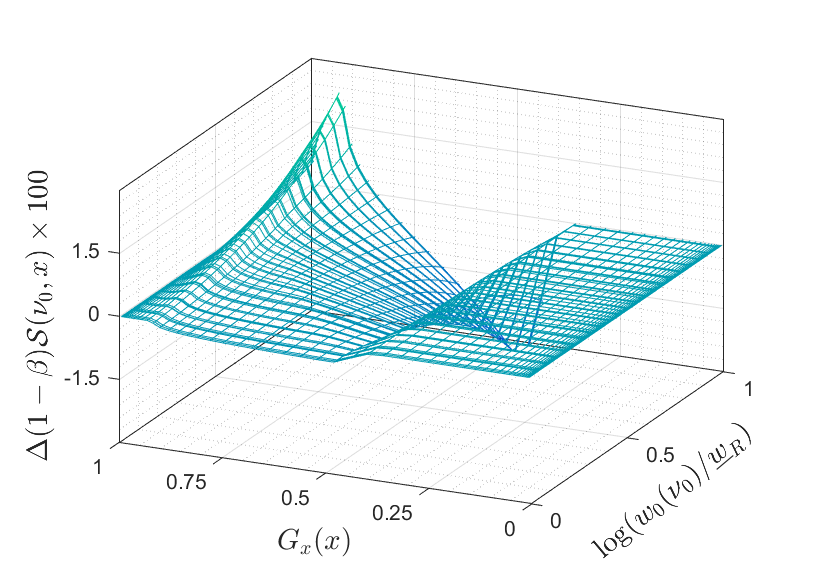
\includegraphics[width=\textwidth]{panel_a.eps}
			\label{fig:panel_a}
		\end{subfigure}
		\begin{subfigure}{0.445\textwidth}
			\centering
			\caption{Equilibrium simulated distributions}
			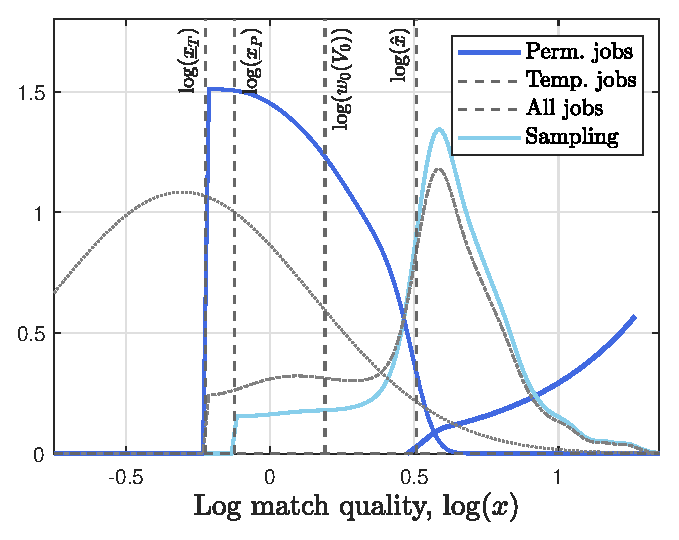
\includegraphics[width=\textwidth]{panel_b.eps}
			\label{fig:panel_d}
		\end{subfigure}
		\begin{subfigure}{0.475\textwidth}
			\centering
			\caption{Matching surplus vs.\ match quality}
			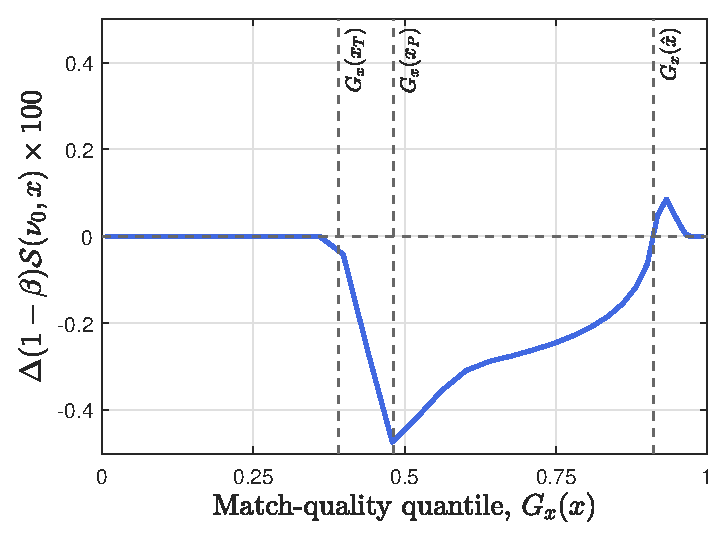
\includegraphics[width=\textwidth]{panel_c.eps}
			\label{fig:panel_d}
		\end{subfigure}
		\begin{subfigure}{0.475\textwidth}
			\centering
			\caption{Matching surplus vs.\ wage}
			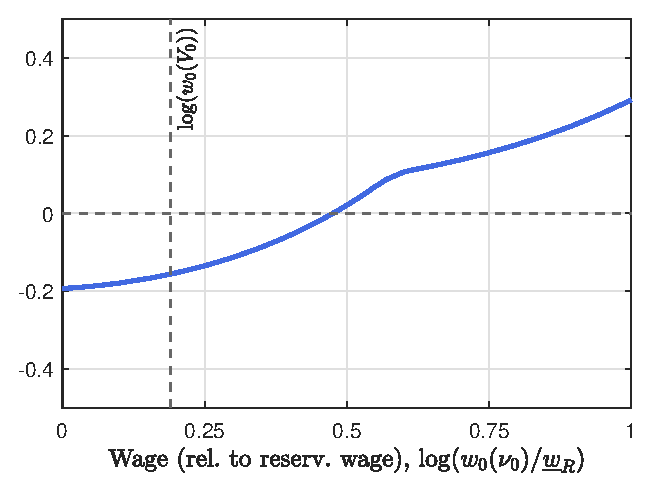
\includegraphics[width=\textwidth]{panel_d.eps}
			\label{fig:panel_d}
		\end{subfigure}
		\caption{Equilibrium outcomes in the ``French'' counterfactual economy}
		\label{fig:eql_outcomes}
		\caption*{\footnotesize Notes: Equilibrium policy and distribution functions in the French-type calibrated economy. Panel a): Hiring surplus difference between a PC and a TC in equivalent annuity consumption terms, $(1-\beta) \Delta \mathcal{S}$ (see equation \eqref{surplus_difference}, versus (i) match-quality quantiles associated with the match quality sampling distribution $G_x(x)$ and (ii) the worker's initial matching values $\nu_0$ in terms of the ``target'' hiring wage $w_0$ (Proposition \ref{proposition:choice})  relative to the reservation wage $w_R \equiv u^{-1}\big[ (1-\beta) U\big]$. Panel b): Gaussian kernel density estimates (bandwidth 0.1) of simulated equilibrium distributions and the sampling distribution of the log match quality $g_x$. The vertical lines show hiring cutoffs $\underline{x}_T$, $\underline{x}_P$, and $\hat{x}$ of Proposition \ref{proposition:choice}. Panel c): Hiring surplus difference between contracts, $(1-\beta) \Delta \mathcal{S}$, evaluated at the equilibrium bargained worker's matching value $V_0$ (which satisfies \eqref{eql:V0}, solution to \eqref{eql:barg_pb}), versus match-quality quantiles. The vertical dashed lines show quantiles associated with the hiring cutoffs of Proposition \ref{proposition:choice}. Panel d): Hiring surplus difference evaluated at a match quality fixed to a value in the interval delimited by hiring cutoffs $[x_P, \hat{x}]$, versus the worker's initial matching values $\nu_0$ (and the associated wage). The vertical dashed line shows the worker's bargained matching value satisfying \eqref{eql:V0} in equilibrium.}
	\end{figure}
	
	\newpage
	
	\setcounter{table}{0}  
	\renewcommand{\thetable}{A\arabic{table}}
	
	\begin{table}[!h]
\centering
\captionof{table}{Decomposition of differences between the French and U.S.\ economies}
\label{tab:France_vs_Spain} 
\begin{tabular}{l c c c c c}
\hline \hline
\addlinespace
 \hspace{100pt} &    Total  & $A$ & $\delta$ & $b$ & $F$   \\
 \addlinespace
 Reference param.\ value (U.S.) & &0.60&0.0024&0.38&0\\
 Comparison param.\ (France) & &0.30&0.0008&0.50&1.37\\
 Param.\ differential &  &-0.30&-0.0016&0.12&1.37\\
 \addlinespace
 \multicolumn{6}{l}{\textit{Labor-market stocks differential (percentage-point)}}  \\
 \hspace{5pt} Unem.\ rate &3.57&0.70&4.93&0.63&3.62\\
 \addlinespace
 \textit{Transition rates (p.p.)}  &   &   &   &   &  \\
 \hspace{5pt} UE           &-21.77&-4.55&-21.25&-12.51&-21.63\\
 \hspace{5pt} EU           &-0.81&-0.33&-0.29&-1.08&-0.78\\
\addlinespace
\hline \hline
\end{tabular}
\caption*{ \footnotesize Notes: Decomposition of differences in aggregate equilibrium outcomes between the ``French'' and U.S.\ baseline model economy. The first column reports the total difference in equilibrium outcomes between these two economies. The subsequent columns report the difference in outcomes after counterfactually imposing a given parameter in the U.S.\ baseline to be equal to its counterpart in the French economy, i.e., a measure of the total difference in equilibrium outcomes attributable to this parameter. The parameters under focus are the matching efficiency $A$ , the exogenous probability of separation $\delta$, the non-work income level $b$, and firing costs $F$. The first row indicates parameter values in the baseline (U.S.) reference economy. The second row indicates the difference in parameter values between the baseline and French model economies. }
\end{table} 
	
	\begin{table}[!h]
\centering
\captionof{table}{Decomposition of differences between the French and Spanish economies}
\label{tab:France_vs_Spain} 
\begin{tabular}{l c c c c c}
\hline \hline
\addlinespace
 \hspace{100pt} &    Total  & $\delta$ & $b$ & $F$ & $\phi$   \\
 \addlinespace
 Reference param.\ value (French) & &0.0008&0.50&1.37&0.045\\
 Comparison param.\ (Spanish) & &0.0019&0.53&1.65&0.030\\
 Param.\ differential &  &0.0011&0.03&0.28&-0.015\\
 \addlinespace
 \multicolumn{6}{l}{\textit{Labor-market stocks differential (percentage-point)}}  \\
 \hspace{5pt} Unem.\ rate &4.32&1.86&2.96&4.30&3.92\\
 \hspace{5pt} TC emp.\ share           &7.52&4.48&6.62&7.47&4.46\\
 \addlinespace
 \textit{Transition rates (p.p.)}  &   &   &   &   &  \\
 \hspace{5pt} UE           &-0.97&-0.92&-0.06&-0.94&-0.98\\
 \hspace{5pt} EU           &0.50&0.14&0.41&0.49&0.44\\
\addlinespace
\hline \hline
\end{tabular}
\caption*{ \footnotesize Notes: Decomposition of differences in aggregate equilibrium outcomes between the ``French'' and ``Spanish'' model economy. The first column reports the total difference in equilibrium outcomes between these two economies. The subsequent columns report the difference in outcomes after counterfactually imposing a given parameter in the French model economy to be equal to its counterpart in the Spanish economy, i.e., a measure of the total difference in equilibrium outcomes attributable to this parameter. The parameters under focus are the exogenous probability of separation $\delta$, the non-work income level $b$, firing costs $F$, and the regulatory restriction on the duration of temporary contracts, $\phi$. The first row indicates parameter values in the French reference economy. The second row indicates the difference in parameter values between the Spanish and French model economies. }
\end{table} 
	
	\newpage
	
	\bibliographystyle{chicago}
	\bibliography{bibliography}
	
\end{document}